% !TEX root = ../waves.tex
%%%%%%%%%%%%%%%%%%%%%%%%%%%%%%%%%%%%%%%%%%%%%%%%%%%%%%%%%%%%%%%%%%%%%%%%%%%%%%%%%%%%%%%%%%
A key property of the Fourier transform is that it transforms derivatives into powers, as
stated in~\cref{prop:ft-trans,prop:ft-der-distrib}:
\begin{equation}
  \mathcal{F}(F^{(\alpha)})(\omega)=(2\pi i\omega)^{\alpha}\hat{F}(\omega)\,,
\end{equation}
where $F$ is a distribution and $\alpha$ is a non-negative integer. We also previously saw
a similar property for Fourier series, \cf\cref{prop:fourier-coef-trans}. We have used this
property several times already to discuss the decay rate of the Fourier coefficients, or
Fourier transform, of a function. Another key application is differential equations, which
in some cases can be considerably simplified by using the formula above.

%%%%%%%%%%%%%%%%%%%%%%%%%%%%%%%%%%%%%%%%%%%%%%%%%%%%%%%%%%%%%%%%%%%%%%%%%%%%%%%%%%%%%%%%%%
\section{Linear ordinary differential equations}
%-----------------------------------------------------------------------------------------
We start with ordinary differential equations, \ie differential equations for which the
unknown function is in one real variable.
\subsection{Homogeneous equations}
We first discuss how to systematically solve any linear homogeneous equation with constant
coefficients. \emph{Homogeneous equations} are differential equations with a zero
right-hand side. The method presented here is called the \emph{characteristic equation
method}. Although it is not necessary, this method can be entirely justified using Fourier
analysis, as we do below. Some properties used are non-trivial, and therefore we use a
mainly heuristic presentation, starting with the well-known cases of the first and
second-order equations.
%.........................................................................................
\subsubsection{Introduction: first-order equation}
Let us start with a simple, well-understood case: the first-order linear equation
\begin{equation}
  y'+ay=0\,,\label{eq:ode1}
\end{equation}
where $a\in\R$. It is well-known that the solutions of this equation are given by
\begin{equation}
  y(t)=C\,e^{-at}\,,
  \label{eq:ode1-sol}
\end{equation}
where $C\in\R$ is a constant that is generally determined using a given initial condition.
Let us see how this result can be re-derived using Fourier analysis. Computing the Fourier
transform on both sides of \cref{eq:ode1}, one obtains
\begin{equation}
  (2\pi i\omega+a)\,\hat{y}(\omega)=0\,.
  \label{eq:ode1-ft}
\end{equation}
Since $a$ is real, $2\pi i\omega+a\neq 0$, and therefore $\hat{y}(\omega)=0$ for all
$\omega$. This naively seems inconsistent with \cref{eq:ode1-sol}. One limitation of the
Fourier transform is that it can only describe functions with moderate growth, and
\cref{eq:ode1-sol} has exponential growth. What we found is the only solution with
moderate growth, which is correctly \cref{eq:ode1-sol} with $C=0$. It is somewhat
disappointing that Fourier analysis seems to fail in solving the simplest differential
equation. However, as we will see, the solution \cref{eq:ode1-sol} can be obtained, just
not directly.

Let us assume more generally that $a$ is a complex number. If $a$ is purely imaginary, \ie
there exists a real number $\alpha$ such that $a=i\alpha$, then $2\pi i\omega+a=0$ for
$\omega=\omega_0$ with $\omega_0=-\frac{\alpha}{2\pi}$. Still, for all
$\omega\neq\omega_0$, \cref{eq:ode1-ft} implies $\hat{y}(\omega)=0$. If we assume
$\hat{y}$ is a standard function, the previous statement once more implies that $y=0$,
since the value of $\hat{y}$ at a single point is irrelevant when taking the inverse
Fourier transform. However, this is not the only possibility if $\hat{y}$ is a
distribution. Indeed, if, for example,
\begin{equation}
  \hat{y}(\omega)=C\,\delta(\omega-\omega_0)\,,
  \label{eq:ode1-delta}
\end{equation}
for an arbitrary constant $C$, then clearly this satisfies \cref{eq:ode1-ft}. Taking the
inverse Fourier transform, we obtain
\begin{equation}
  y(x)=C\,e^{2\pi i\omega_0t}=C\,e^{-i\alpha t}=C\,e^{-at}\,,
\end{equation}
which is the desired solution. There is still one important limitation: the procedure
above only works for $a$ purely imaginary. However, once the solution above has been
obtained, we can notice it is in fact valid for any complex number $a$, which includes real
values. This extension at the final step is generally referred to as \emph{analytical
continuation}.

The procedure above might look quite convoluted to obtain a solution that can be derived
in much simpler ways (\eg separation of variables). It additionally contains a number of
steps that naively look arbitrary:
\begin{enumerate}
  \item Using a delta function in \cref{eq:ode1-delta} solves \cref{eq:ode1-ft}, but is
    this choice unique?
  \item The method was initially limited to $a$ purely imaginary, yet it generated a more
    general solution. Is that generally expected?
\end{enumerate}
Regarding point 1, there is indeed a non-trivial characterisation of distributions that
vanish everywhere except at one point, which implies that the delta function was a unique
solution. We will discuss that explicitly in the next part of this section. For point 2,
it is generally expected that such continuation is possible if the Fourier transform of
$y$ vanishes everywhere except at a finite number of points. This is a non-trivial result,
which relates the Fourier transform to a similar operation called the \emph{Laplace
transform}. We will admit that such continuation is expected. In practice, one can always
attempt such extension, and check using the differential equation that new solutions are
obtained. Let us now discuss point 1 in detail.
%.........................................................................................
\subsubsection{Structure theorem}
We start by stating the following \emph{structure theorem}. This is a highly non-trivial
result that will be admitted here.
\begin{theorem}
  \label{thm:structure}
  Let $f$ be a smooth moderately growing function on $\R$, which admits a unique zero at
  $x_0\in\R$. Let $F$ be a distribution on $\R$ such that
  \begin{equation}
    F(x)f(x)=0\,,
  \end{equation}
  in the sense of distributions. Then there exist a finite number $N+1$ of complex numbers
  $c_n$ such that
  \begin{equation}
    F(x)=\sum_{n=0}^{N}c_n\,\delta^{(n)}(x-x_0)\,.
  \end{equation}
\end{theorem}
So if a distribution is zero everywhere except at one point, then it must be a linear
combination of the delta function and its derivatives at this point. If a function cancels
at a finite number of points, then each zero can contribute delta functions (and
derivatives) to $F$. In the previous case of \cref{eq:ode1-ft}, we did not consider
derivatives as possible solutions, which we will now justify. The theorem above can be
specialised for polynomials, where the highest possible derivative of the delta function
contributing to $F$ is associated with the multiplicity of the associated root:
\begin{theorem}
  \label{thm:structure-poly}
  Let $P(x)$ be a polynomial that admits a real root of multiplicity $d$ at $x=x_0$. Let
  $F$ be a distribution on $\R$ such that
  \begin{equation}
    F(x)P(x)=0\,,
    \label{eq:prodzero-poly}
  \end{equation}
  in the sense of distributions. Then there exist $d$ complex numbers $c_n$ such that
  \begin{equation}
    F(x)=\sum_{n=0}^{d-1}c_n\,\delta^{(n)}(x-x_0)\,.
  \end{equation}
\end{theorem}
\begin{proof}
  If $x_0$ is a real root of multiplicity $d$ of $P(x)$, then there exists a polynomial
  $Q(x)$ such that
  \begin{equation}
    P(x)=(x-x_0)^dQ(x)\qquad\text{and}\qquad Q(x_0)\neq 0\,.\label{eq:poly-factor}
  \end{equation}
  Using \cref{thm:structure}, we know that there exist $N+1$ complex numbers $c_n$ such
  that
  \begin{equation}
    F(x)=\sum_{n=0}^{N}c_n\,\delta^{(n)}(x-x_0)\,.
  \end{equation}
  For the sake of simplicity, let us prove the theorem for $d=1$ first. In this case, we
  have
  \begin{equation}
    P'(x)=Q(x)+(x-x_0)Q'(x)\,,
  \end{equation}
  and therefore
  \begin{equation}
    P'(x_0)=Q(x_0)\neq 0\,.
  \end{equation}
  Using~\cref{eq:deltan-times-f}, $\delta^{(n)}(x-x_0)P(x)$ will always contain a non-zero
  term if $n\geq 1$ (\ie the term with $j=1$ in \cref{eq:deltan-times-f}). So in order to
  satisfy~\cref{eq:prodzero-poly}, we must have $N=0$, \ie $F$ can only be proportional to
  the delta function. The case of arbitrary multiplicity is similar. One can show that
  there exists a polynomial $R(x)$ such that
  \begin{equation}
    P^{(d)}(x)=d!Q(x)+(x-x_0)R(x)\,,
  \end{equation}
  obtained by taking $d$ derivatives of \cref{eq:poly-factor}. Therefore,
  $P^{(d)}(x_0)\neq 0$, and $\delta^{(n)}(x-x_0)P(x)\neq 0$ if $n\geq d$. So necessarily
  $N<d$ and the theorem is proven.
\end{proof}
Returning to~\cref{eq:ode1-ft}, the polynomial $2\pi i\omega +a$ has degree $1$, and for
$a=i\alpha$ it has one real root of multiplicity $1$, so $\hat{y}$ must be proportional to
the delta function. Let us now apply these results to the case of the second-order
equation.
%.........................................................................................
\subsubsection{Undamped second-order equation}
We start by considering the second-order equation for the undamped harmonic oscillator:
\begin{equation}
  y''+ay=0\,,
\end{equation}
where $a\in\R$. The Fourier transform of this equation gives
\begin{equation}
  P(\omega)\hat{y}(\omega)=0,\qquad\text{with}\qquad P(\omega)=-4\pi^2\omega^2+a\,.
\end{equation}
$P(\omega)$ is a degree 2 polynomial with the following root structure:
\begin{itemize}
  \item If $a>0$, $P(\omega)$ has two real single roots
    $\omega_{\pm}=\pm\frac{\sqrt{a}}{2\pi}$;
  \item If $a=0$, $P(\omega)$ has a real double root at $\omega=0$;
  \item If $a<0$, $P(\omega)$ has two complex roots $\omega_{\pm}$.
\end{itemize}
Using \cref{thm:structure-poly}, if $a>0$, there exist two constants $A$ and $B$ such
that
\begin{equation}
  \hat{y}(\omega)=A\,\delta(\omega-\omega_-)+B\,\delta(\omega-\omega_+)\,,
\end{equation}
and therefore
\begin{equation}
  y(t)=A\,e^{2\pi i\omega_+t}+B\,e^{2\pi i\omega_-t}=A\,e^{i\sqrt{a}t}+B\,e^{-i\sqrt{a}t}\,,
  \label{eq:ode2-periodic}
\end{equation}
which can be written in the more usual form
\begin{equation}
  y(t)=\alpha\cos(\sqrt{a}t)+\beta\sin(\sqrt{a}t)\,,
\end{equation}
with $\alpha=A+B$ and $\beta=i(A-B)$. In this case, the solution is periodic and could
have been obtained with a Fourier series expansion, \cf\cref{fourierode2}.

Now, if $a=0$, $y''=0$, and clearly $y$ is linear. But let us use \cref{thm:structure-poly}
regardless: since $\omega=0$ is a double root of $P(\omega)$, there exist two constants
$A$ and $B$ such that
\begin{equation}
  \hat{y}(\omega)=A\,\delta(\omega)+B\,\delta'(\omega)\,,
\end{equation}
which has the inverse Fourier transform
\begin{equation}
  y(t)=A-2\pi i Bt\,,
\end{equation}
which is the expected linear result.

Finally, if $a<0$, $P(\omega)$ has no real roots and, strictly speaking, the only solution
coming from the Fourier transform is zero. However, as we did in the first-order case, we
can analytically continue the result obtained in~\cref{eq:ode2-periodic} to the two
complex roots of $P(\omega)$, which leads to the potential solution
\begin{equation}
  y(t)=A\,e^{-\sqrt{a}t}+B\,e^{\sqrt{a}t}\,.
  \label{eq:ode2-exp}
\end{equation}
One can easily check that the continuation above is indeed a solution. Once again, this
solution cannot be found directly using a Fourier transform since it contains
exponentially growing terms. As we can see, the method described in this section
reconstructs easily the well-known three classes of solutions for this equation, without
prior knowledge. Let us now look at the case of the damped oscillator.
%.........................................................................................
\subsubsection{Damped second-order equation}
The damped harmonic oscillator equation is given by:
\begin{equation}
  y''+2aby'+a^2y=0\,,
\end{equation}
where $a$ and $b$ are positive real numbers. This equation has the Fourier form
\begin{equation}
  \label{eq:ode2-damped-ft}
  P(2\pi i\omega)\hat{y}(\omega)=0,\qquad\text{with}\qquad
  P(s)=s^2+2sab+a^2\,.
\end{equation}
As we saw in the previous cases, specifically in~\cref{eq:ode2-periodic,eq:ode2-exp}, the
roots of the polynomial appearing in the Fourier-transformed equation always end up being
multiplied by $2\pi i$ in the solution. Therefore, it is generally simpler to arbitrarily
consider a polynomial in the variable $s=2\pi i\omega$. The variable $s$ is sometimes
called \emph{in the Laplace domain}; it is an imaginary frequency in contrast with
$\omega$, which is said to be \emph{in the Fourier domain}. The polynomial $P(s)$ can be
factorised as follows
\begin{equation}
  P(s)=(s+ab)^2+a^2(1-b^2)\,,
\end{equation}
which leads to the three cases:
\begin{itemize}
  \item If $b<1$, $P(s)$ has two single complex roots
    \begin{equation}
      s_{\pm}=-ab\pm ia\sqrt{1-b^2}\,.
    \end{equation}
  \item If $b>1$, $P(s)$ has two single real roots
    \begin{equation}
      \bar{s}_{\pm}=-ab\pm a\sqrt{b^2-1}\,.
    \end{equation}
  \item If $b=1$, $P(s)$ has one double real root at $s_0=-a$.
\end{itemize}
In all cases, all roots in the Fourier domain are purely complex, and therefore the
equation \cref{eq:ode2-damped-ft} systematically leads to the trivial solution $y=0$.
However, clearly all roots above could be made real if one would consider complex values
for $a$ and $b$, and one can try to use analytical continuation. So, treating roots as if
they were real, we obtain
\begin{enumerate}
  \item If $b<1$, there exist two constants $A$ and $B$ such that
    \begin{equation}
      \hat{y}(\omega)=A\,\delta(\omega-\omega_+)+B\,\delta(\omega-\omega_-)\,,
    \end{equation}
    with $2\pi i\omega_{\pm}=s_\pm$, and therefore
    \begin{align}
      y(t)&=A\,e^{2\pi i\omega_+ t}+B\,e^{2\pi i\omega_- t}
      =A\,e^{s_+ t}+B\,e^{s_- t}
      \notag\\
      &=A\,e^{-abt}e^{ia\sqrt{1-b^2}t}+B\,e^{-abt}e^{-ia\sqrt{1-b^2}t}\notag\\
      &=e^{-abt}[\alpha\cos(a\sqrt{1-b^2}t)+\beta\sin(a\sqrt{1-b^2}t)]\,,
      \label{eq:ode2-damped-under}
    \end{align}
    with $\alpha=A+B$ and $\beta=i(A-B)$. This is the \emph{underdamped regime}, with
    oscillations decaying exponentially fast.
  \item If $b>1$, there exist two constants $A$ and $B$ such that
    \begin{equation}
      \hat{y}(\omega)=A\,\delta(\omega-\bar{\omega}_+)+B\,\delta(\omega-\bar{\omega}_-)\,,
    \end{equation}
    with $2\pi i\bar{\omega}_{\pm}=\bar{s}_\pm$, and therefore
    \begin{align}
      y(t)&=A\,e^{2\pi i\bar{\omega}_+ t}+B\,e^{2\pi i\bar{\omega}_- t}
      =A\,e^{\bar{s}_+ t}+B\,e^{\bar{s}_- t}\notag\\
      &=A\,e^{-(ab+a\sqrt{b^2-1})t}+B\,e^{-(ab-a\sqrt{b^2-1})t}\,.
      \label{eq:ode2-damped-over}
    \end{align}
    Clearly $ab\pm a\sqrt{b^2-1}>0$, and this solution is decaying exponentially fast for
    $t\to+\infty$. This case is called the \emph{overdamped regime}.
  \item Finally, if $b=1$, there exist two constants $A$ and $B$ such that
    \begin{equation}
      \hat{y}(\omega)=A\,\delta(\omega-\omega_0)+B\,\delta'(\omega-\omega_0)\,,
    \end{equation}
    with $2\pi i\omega_{0}=s_0$, and therefore
    \begin{equation}
      y(t)=(A-2\pi i Bt)\,e^{s_0 t}
      =(A-2\pi i Bt)\,e^{-at}\,.
      \label{eq:ode2-damped-crit}
    \end{equation}
    This is the \emph{critically damped regime}.
\end{enumerate}
We can now formulate the general case for an arbitrary order $n$ equation.
%.........................................................................................
\subsubsection{General case}
We consider the order $n$ homogeneous equation
\begin{equation}
  a_ny^{(n)}+\cdots+a_1y'+a_0y=0\,,\label{eq:oden}
\end{equation}
where the $a_j$ for $0\leq j\leq n$ are complex numbers such that $a_n\neq 0$.
Generalising previous examples, this equation can be solved using the two steps described
below.
\begin{enumerate}
  \item The polynomial
    \begin{equation}
      P(s)=\sum_{j=0}^{n} s^ja_j\,,
    \end{equation}
    is called the \emph{characteristic polynomial} of \cref{eq:oden}. It is defined such
    that
    \begin{equation}
      P(2\pi i\omega)\hat{y}(\omega)=0\,,
    \end{equation}
    for all frequencies $\omega\in\R$. The first step is to determine the roots of $P(s)$.
    Since $P(s)$ is of degree $n$, it has $n$ complex roots, with potential degeneracies.
    We note $s_j$, with $1\leq j\leq r$, the \emph{distinct} roots of $P(s)$. Naturally,
    $r\leq n$, and we note $m_j$ the multiplicity of root $s_j$.
  \item Each root contributes
    \begin{equation}
      y_j(t)=(C_{j,1}+\cdots+C_{j,m_j}t^j)\,e^{s_jt}
    \end{equation}
    to the solution, where $C_{j,1},\dots,C_{j,m_j}$ are $m_j$ arbitrary integration
    constants that need to be determined using initial conditions. The general solution of
    \cref{eq:oden} is then given by
    \begin{equation}
      y(t)=\sum_{j=1}^{r}y_j(t)\,,
    \end{equation}
    and is parametrised by a total of $n$ integration constants. For each $j$, the real
    part of $s_j$ contributes an exponentially varying term, and the imaginary part an
    oscillatory term.
\end{enumerate}
%.........................................................................................
\subsubsection{Non-constant coefficients}
When coefficients are not constant, solving systematically a linear differential equation,
even in the homogeneous case, is non-trivial. However, the Fourier transform of an
equation can in some cases lead to an easier equation to solve. We refer the reader to
\cref{airy} for an explicit example with the Airy equation. We now discuss the case of
inhomogeneous equations.
%-----------------------------------------------------------------------------------------
\subsection{Inhomogeneous equations}
\label{sec:ih-ode}
In the inhomogeneous case, equations can have an arbitrary function on their right-hand
side. Physically, the right-hand side often represents an external interaction term on
the system, \eg a driving force in the case of oscillators. Fourier analysis provides a
systematic way of solving this case using Green's function, which is a crucial method in
numerous physical applications. Let us first describe the general method.
%.........................................................................................
\subsubsection{General case -- Green's function}
We consider the inhomogeneous equation
\begin{equation}
  a_ny^{(n)}(t)+\cdots+a_1y'(t)+a_0y(t)=f(t)\,,\label{eq:oden-nonh}
\end{equation}
where $f$ is an arbitrary moderately growing function. Firstly, one can observe that if
$y$ is a particular solution of the equation above, and if $y_0$ is a solution of the
associated homogeneous equation \cref{eq:oden}, then clearly $y+y_0$ is also a solution of
the inhomogeneous equation. In fact, one can prove that this procedure spans the entire
set of solutions for the inhomogeneous equation. The Fourier domain equation is given by
\begin{equation}
  P(2\pi i\omega)\hat{y}(\omega)=\hat{f}(\omega)\,,
\end{equation}
where $P$ is the characteristic polynomial as defined in the previous section. Therefore,
a particular solution of \cref{eq:oden-nonh} is given by
\begin{equation}
  y_P(t)=\intr{\omega}\frac{\hat{f}(\omega)}{P(2\pi i\omega)}\,e^{2\pi i \omega t}\,.
  \label{eq:oden-part}
\end{equation}
The inverse Fourier transform above is in the sense of distributions, and special care
might be needed if $P(2\pi i\omega)$ has real roots in $\omega$, which generate
singularities in the integrand above.

There is a standard way in physics to express the solution above. First, one defines the
\emph{Green's function} $G$, sometimes also called \emph{fundamental solution}, as the
solution of~\cref{eq:oden-nonh} for $f(t)=\delta(t)$. Since the Fourier transform of the
delta function is $1$, clearly
\begin{equation}
  \hat{G}(\omega)=\frac{1}{P(2\pi i\omega)}\qquad\text{and}\qquad
  G(t)=\intr{\omega}\frac{1}{P(2\pi i\omega)}\,e^{2\pi i \omega t}\,.
  \label{eq:green-ft}
\end{equation}
Then, the particular solution for a general right-hand side \cref{eq:oden-part} can be
written
\begin{equation}
  \label{eq:oden-part-conv}
  y_P(t)=\intr{\omega}\hat{G}(\omega)\hat{f}(\omega)\,e^{2\pi i\omega t}
  =(G\ast f)(t)\,.
\end{equation}
Finally, the general solution of \cref{eq:oden-nonh} is given by
\begin{equation}
  y(t)=(G\ast f)(t)+y_0(t)\,,
\end{equation}
where $y_0$ is a solution of the homogeneous equation~\cref{eq:oden} that should be fixed
using initial conditions.
%.........................................................................................
\subsubsection{Driven harmonic oscillator}
We consider a mass $m$ attached to a spring fixed at one end along the horizontal axis, at
position $x=0$. We denote by $x(t)$ the position of the mass on the horizontal axis as a
function of time $t$. Furthermore, we assume the mass is driven by an external force
$F(t)$ varying with time, and that it is insensitive to gravity (\eg it is mounted on a
horizontal rail). In total, three forces are applied to the mass:
\begin{itemize}
  \item The spring restoration force $F_s=-kx$ (Hooke's law);
  \item A friction force opposite to the velocity $F_f=-cx'$;
  \item The external time-varying force $F$.
\end{itemize}
Above, $k>0$ is the spring constant in $\newton\per\metre$, and $c>0$ is the friction
coefficient in $\newton\usk\second\per\metre$. Applying Newton's second law, we obtain the
differential equation
\begin{equation}
  mx''=F_s+F_f+F=-cx'-kx+F\,,
\end{equation}
which is commonly put in the form
\begin{equation}
  x''+4\pi\zeta\omega_0x'+4\pi^2\omega_0^2x=\frac{F}{m}\,,\label{eq:ode2-driven}
\end{equation}
where $\omega_0=\smash{\frac{1}{2\pi}\sqrt{\frac{k}{m}}}$ is the \emph{undamped frequency}
in $\hertz$, and $\zeta=\smash{\frac{c}{2\sqrt{mk}}}$ is the \emph{damping ratio}, which
is a dimensionless number. We already solved the homogeneous equation in the previous
section, \cf\cref{eq:ode2-damped-under,eq:ode2-damped-over,eq:ode2-damped-crit}, with
$a=2\pi\omega_0$ and $b=\zeta$.

We now want to find particular solutions of the inhomogeneous equation. This can be
done by finding the Green's function $G$ of~\cref{eq:ode2-driven}. Following
\cref{eq:green-ft},
\begin{equation}
  G(t)=\intr{\omega}\frac{e^{2\pi i\omega t}}{P(2\pi i\omega)}\,,
\end{equation}
with the characteristic polynomial $P(s)=s^2+4\pi\zeta\omega_0s+4\pi^2\omega_0^2$. The
traditional way of computing explicitly such Fourier transform is to use complex analysis
and contour integration. However, we will not assume here that the reader is familiar with
this formalism and provide an alternative way of computing $G$.

Let us assume we are in the underdamped regime, \ie $\zeta<1$. Then we know that
\begin{equation}
  P(s)=(s-s_+)(s-s_-)\qquad\text{with}\qquad
  s_\pm=-2\pi\omega_0\zeta\pm 2\pi i\omega_1\,,
\end{equation}
where $\omega_1=\omega_0\sqrt{1-\zeta^2}$ is the \emph{damped frequency} of the
oscillator. We then write
\begin{equation}
  \frac{1}{P(2\pi i\omega)}=\frac{1}{4\pi i\omega_1}\left(\frac{1}{2\pi i\omega-s_+}
  -\frac{1}{2\pi i\omega-s_-}\right)\,.
  \label{eq:p-part-frac}
\end{equation}
We can compute the inverse Fourier transforms of the terms above, which have the general
form
\begin{equation}
  \intr{\omega}\frac{e^{2\pi i\omega t}}{2\pi i \omega-z}\,,
\end{equation}
where $z$ is a complex number such that $\Re(z)<0$. A useful and simple identity,
sometimes referred to as the \emph{Schwinger parameterisation}, is as follows:
\begin{equation}
  \frac{1}{A}=\int_0^{+\infty}\diff\lambda\,e^{-\lambda A}
  =\intr{\lambda}\theta(\lambda)e^{-\lambda A}\,,
\end{equation}
where $A$ is a complex number such that $\Re(A)>0$. Since $\Re(z)<0$, $\Re(2\pi i
\omega-z)>0$, and therefore using the Schwinger parameterisation
\begin{align}
  \intr{\omega}\frac{e^{2\pi i\omega t}}{2\pi i \omega-z}&=
  \intr{\omega}\intr{\lambda}\theta(\lambda)
  e^{2\pi i\omega(t-\lambda)}e^{\lambda z}\notag\\
  &=\intr{\lambda}\theta(\lambda)\delta(t-\lambda)e^{\lambda z}\notag\\
  &=\theta(t)e^{zt}\,.
  \label{eq:thetaexp}
\end{align}
Applying this result to \cref{eq:p-part-frac}, we finally obtain
\begin{equation}
  \boxed{G(t)
  =\theta(t)e^{-2\pi\omega_0\zeta t}\,\frac{\sin(2\pi\omega_1t)}{2\pi\omega_1}}\,.
  \label{eq:green-underdamped}
\end{equation}
Following similar steps, one obtains in the $\zeta>1$ overdamped regime
\begin{equation}
  \boxed{
    G(t)=\theta(t)e^{-2\pi\omega_0\zeta t}\,
  \frac{\sinh(2\pi\bar{\omega}_1t)}{2\pi\bar{\omega}_1}}\,,
  \label{eq:green-overdamped}
\end{equation}
where $\bar{\omega}_1=\omega_0\sqrt{\zeta^2-1}$. In the critical $\zeta=1$ regime, one has
\begin{equation}
  \boxed{G(t)=\theta(t)te^{-2\pi\omega_0 t}}\,.
  \label{eq:green-critical}
\end{equation}
The derivation of these extra cases is left to the reader as an exercise
(\cf\cref{green}). The Green's function $G$ in the three regimes above is represented in
\cref{fig:ho-green}. We now discuss the physical interpretation of these objects.
\begin{figure}[t]
  \centering
  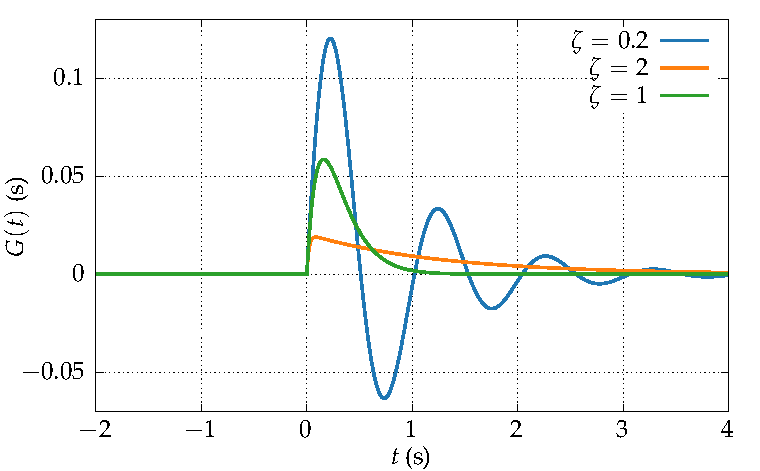
\includegraphics{gp_ho-green.pdf}
  \caption{Green's function of the damped harmonic oscillator in the underdamped,
    overdamped, and critical regimes for an undamped frequency $\omega_0=\unit{1}{\hertz}$.
    The explicit form of $G(t)$ is given in
  \cref{eq:green-underdamped,eq:green-overdamped,eq:green-critical}.}
  \label{fig:ho-green}
\end{figure}
%.........................................................................................
\subsubsection{Physical interpretation of the Green's function}
Let us discuss the physical interpretation of the Green's function. First we consider its
physical dimensions: $G$ is the solution of
\begin{equation}
  G''(t)+4\pi\zeta\omega_0 G'(t)+4\pi^2\omega_0^2G(t)=\delta(t)\,.
\end{equation}
Firstly, the delta function has the inverse dimension of its argument. This can be seen,
for example, using the approximation of $\delta$ by a Gaussian kernel. So $\delta(t)$ is
an inverse time. Since $\omega_0$ is also an inverse time, the equation above implies that
$G(t)$ has the dimension of time. This is dimensionally consistent with
\cref{eq:green-underdamped}. Considering an arbitrary momentum $p$ (in
$\newton\usk\second$), then $\frac{p}{m}G(t)$ is the solution of \cref{eq:ode2-driven}
with the external force $F(t)=p\delta(t)$. So the Green's function is the response of the
oscillator when a momentum $p$ is instantly injected at $t=0$. This is why Green's functions
are also often called \emph{impulse response}, particularly in a signal theory or applied
physics context. With this interpretation in mind, the presence of the Heaviside function
$\theta(t)$ in~\cref{eq:green-underdamped} is not surprising: injecting momentum at $t=0$
only has an effect on the future, \ie for $t>0$. Such a Green's function is called
\emph{retarded} or \emph{causal}. One can observe through the derivation of $G(t)$ that
the $\theta(t)$ factor emerged from the condition $\Re(s_{\pm})<0$, which in turn comes
from $\zeta>0$. In the absence of damping (\ie for $\zeta=0$), one can show that the
definition of $G(t)$ becomes ambiguous, and can influence both future and past, which can
be counter-intuitive. The physical interpretation is that in the presence of damping, the
system loses energy and a clear direction of time is imposed. In the absence of damping,
time reversal becomes a symmetry of the system, and the Green's function can be
interpreted as the future response to an impulse, or the annihilation of a past movement.

Let us now discuss the interpretation of the frequency space Green's function, \ie
\begin{equation}
  \boxed{
    \hat{G}(\omega)=\frac{1}{P(2\pi i\omega)}=\frac{1}{4\pi^2}
  \frac{1}{-\omega^2+2i\zeta\omega_0\omega+\omega_0^2}}\,.
  \label{eq:ho-green-ft}
\end{equation}
In this form, the Green's function describes the response of the oscillator when driven at
a fixed frequency $\omega$. Indeed, for a force $A>0$ in Newtons, we can consider
\cref{eq:ode2-driven} where the external force is an elementary wave with amplitude $A$
and frequency $\omega$, \ie $F(t)=A\cos(2\pi\omega t)$. Then we know that a particular
solution of the equation is given by convoluting $F$ with the Green's function, leading to
\begin{equation}
  y_P(t)=\frac{1}{m}(F\ast G)(t)=\frac{A}{m}\intr{u}G(u)\cos[2\pi\omega(t-u)]\,.
\end{equation}
Using $\cos(x)=\Re(e^{ix})$, and the fact that $G$ is real, we obtain
\begin{equation}
  y_P(t)=\frac{A}{m}\Re\left[\intr{u}G(u)\,e^{2\pi i\omega(t-u)}\right]
  =\frac{A}{m}\Re[\hat{G}(\omega)\,e^{2\pi i\omega t}]\,.
\end{equation}
Let us now write $\hat{G}$ in the polar form
$\hat{G}(\omega)=R(\omega)\,e^{-i\phi(\omega)}$, which gives
\begin{equation}
  y_P(t)=\frac{AR(\omega)}{m}\cos[2\pi\omega t-\phi(\omega)]\,.
\end{equation}
We can make $R$ and $\phi$ more explicit, but before that let us physically interpret the
solution above. If the oscillator is driven by an external oscillation at frequency
$\omega$, the solution above tells us that the oscillator will also oscillate with
frequency $\omega$, although delayed by a phase $\phi(\omega)$. Additionally, this
oscillating movement has an amplitude proportional to $R(\omega)$. $R(\omega)$ is called
the \emph{frequency response} of the oscillator, and $\phi(\omega)$ is the \emph{phase
shift}. Let us compute explicitly these functions using~\cref{eq:ho-green-ft}. We start by
the frequency response
\begin{equation}
  R(\omega)=|\hat{G}(\omega)|=\frac{1}{4\pi^2}
  \frac{1}{\sqrt{(\omega_0^2-\omega^2)^2+4\zeta^2\omega_0^2\omega^2}}
  =\frac{1}{4\pi^2\omega_0^2}\bar{R}\left(\frac{\omega}{\omega_0}\right)\,,
\end{equation}
where $\bar{R}$ is the dimensionless function given by
\begin{equation}
  \boxed{
  \bar{R}(\xi)=\frac{1}{\sqrt{(1-\xi^2)^2+4\zeta^2\xi^2}}\,.}
  \label{eq:ho-response}
\end{equation}
For the phase shift, we first write
\begin{equation}
  \hat{G}(\omega)=\frac{R(\omega)^2}{4\pi^2}(-\omega^2-2i\zeta\omega_0\omega+\omega_0^2)\,,
\end{equation}
therefore $\phi(\omega)$ is such that
\begin{equation}
  \boxed{
    \tan[\phi(\omega)]=\frac{2\zeta\omega_0\omega}{\omega_0^2-\omega^2}
  =\frac{2\zeta\xi}{1-\xi^2}\,,}
  \label{eq:ho-phase}
\end{equation}
where $\xi=\frac{\omega}{\omega_0}$.
\begin{figure}[p]
  \centering
  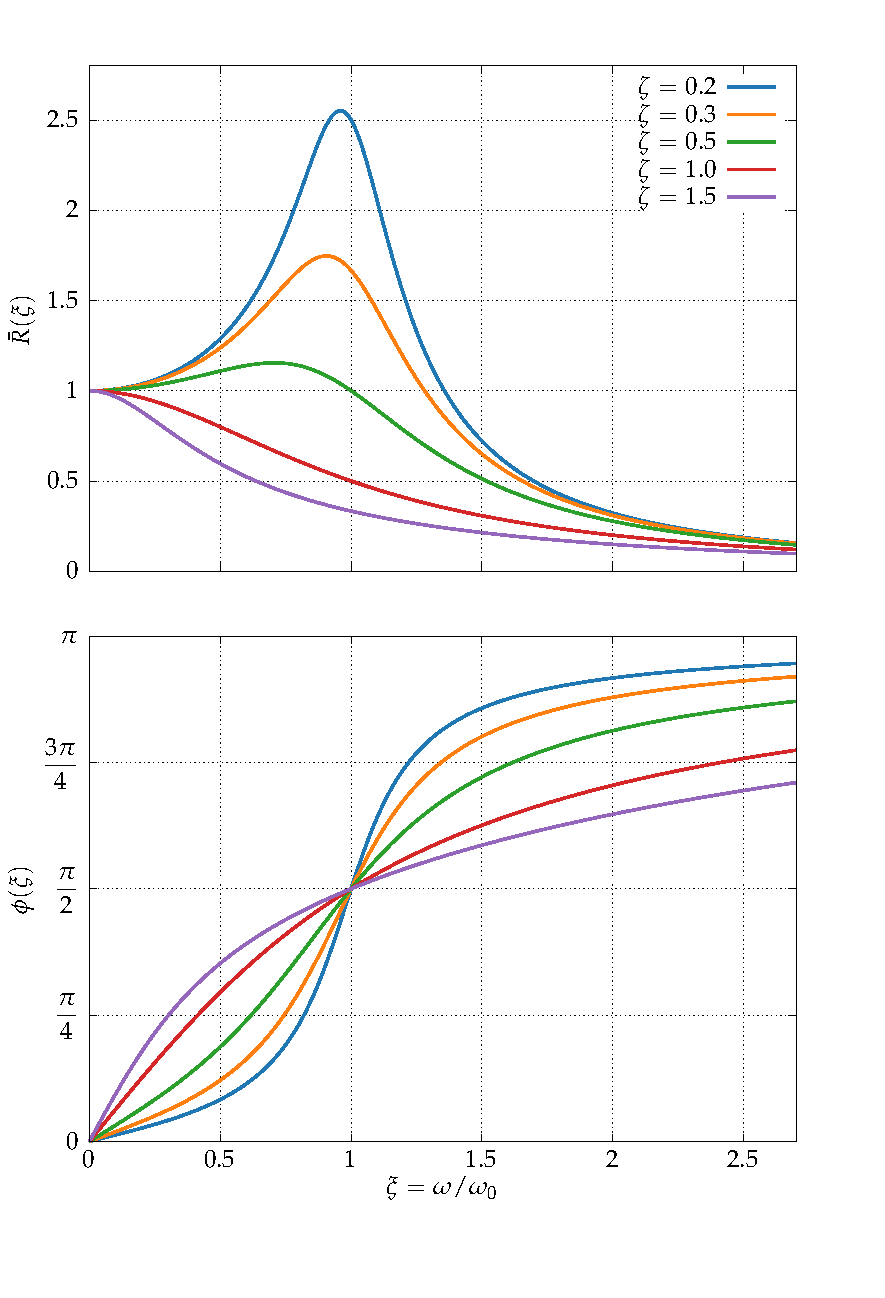
\includegraphics{gp_resonance.pdf}
  \caption{Frequency response (upper pane) and phase shift (lower pane) of the driven
    harmonic oscillator as a function of the frequency ratio $\xi=\frac{\omega}{\omega_0}$,
    where $\omega_0$ is the undamped oscillator frequency. Both functions are defined
    in~\cref{eq:ho-response,eq:ho-phase}, and the phase shift was defined in the
  interval~$[0,\pi)$.}
  \label{fig:resonance}
\end{figure}

The frequency response and phase shift are represented in~\cref{fig:resonance} for various
values of the damping ratio $\zeta$. In the underdamped $\zeta<1$ regime, we clearly
observe that for frequencies around the undamped frequency $\omega_0$, the amplitude of
oscillations is amplified. This is the well-known \emph{resonance} phenomenon which is a
characteristic feature of the driven harmonic oscillator. Regarding the phase shift in the
resonant regime, at frequencies much lower than $\omega_0$, $\phi(\omega)$ is close to
$0$, and at frequencies much higher than $\omega_0$, $\phi(\omega)$ is close to $\pi$.
This can be physically interpreted in the following way: $\omega_0$ is a characteristic
frequency of the oscillator, as it is determined by its mass and spring constant. If the
driver oscillates much slower than this frequency, then the oscillator is able to follow
this movement with a negligible reaction time and is in phase with the driver. However,
if the driver oscillates much faster than $\omega_0$, the reaction time of the oscillator
is too slow to be synchronised, and it is completely out of phase with the driver.
%%%%%%%%%%%%%%%%%%%%%%%%%%%%%%%%%%%%%%%%%%%%%%%%%%%%%%%%%%%%%%%%%%%%%%%%%%%%%%%%%%%%%%%%%%
\section{Partial differential equations}
%-----------------------------------------------------------------------------------------
\subsection{Wave equation}
%.........................................................................................
\subsubsection{Homogeneous equation}
The homogeneous wave equation is given by~\cref{eq:wave-eq}:
\begin{equation}
  \pdn{u}{t}{2}-c^2\,\pdn{u}{x}{2}=0\,.
\end{equation}
For the mechanical string, $x\in[0,L]$ and we have the boundary conditions
\begin{equation}
  u(t,0)=u(t,L)=0\,,
  \label{eq:string-bc-2}
\end{equation}
for all $t\in\R$. For all $x\in[0,L]$, we can consider the Fourier transform in $t$:
\begin{equation}
  \hat{u}(\omega,x)=\intr{t}u(t,x)\,e^{-2\pi i\omega t}\,.
\end{equation}
The wave equation for $\hat{u}$ then becomes
\begin{equation}
  c^2\pdn{\hat{u}}{x}{2}(\omega,x)+4\pi^2\omega^2\hat{u}(\omega,x)=0\,.
\end{equation}
We recognise the undamped harmonic oscillator equation studied in the previous section.
More specifically, we have such an equation in the independent variable $x$ for each value
of $\omega$. Therefore, there exist two constants $A(\omega)$ and $B(\omega)$ such that
\begin{equation}
  \hat{u}(\omega,x)=A(\omega)\cos\left(2\pi\frac{\omega}{c}x\right)+
  B(\omega)\sin\left(2\pi\frac{\omega}{c}x\right)\,.
\end{equation}
Let us now apply the boundary conditions \cref{eq:string-bc-2}; clearly,
$\hat{u}(\omega,0)=\hat{u}(\omega,L)=0$ for all $\omega\in\R$. The condition
$\hat{u}(\omega,0)=0$ directly implies that $A(\omega)=0$ for all $\omega\in\R$. Then, the
second condition $\hat{u}(\omega,L)=0$ implies that
\begin{equation}
  B(\omega)\sin\left(2\pi\frac{\omega}{c}L\right)=0\,.
\end{equation}
This equation can be solved in the sense of distributions using~\cref{thm:structure}. The
sine function above vanishes if and only if $\omega=\frac{cn}{2L}$ for $n\in\Z$, so we
expect $B(\omega)$ to be a linear combination of the delta function and its derivatives at
each of these points. It is not difficult to see that only the delta function can be
present; indeed, for $n\in\Z$,
\begin{align}
  \delta'\left(\omega-\frac{cn}{2L}\right)\sin\left(2\pi\frac{\omega}{c}L\right)&=
  -2\pi\frac{L}{c}\cos\left(2\pi\frac{\omega}{c}L\right)
  \delta\left(\omega-\frac{cn}{2L}\right)\\
  &=2\pi (-1)^{n+1}\frac{L}{c}\delta\left(\omega-\frac{cn}{2L}\right)\neq 0\,,
\end{align}
and this non-zero contribution will be present when multiplying the sine by any higher
derivative of the delta function. So there exists a sequence of complex numbers $C_n$ such
that
\begin{equation}
  B(\omega)=\sumz{n}C_n\,\delta\left(\omega-\frac{cn}{2L}\right)\,,
\end{equation}
and therefore,
\begin{equation}
  \hat{u}(\omega,x)=\frac12\sumz{n}C_n\,\delta\left(\omega-\frac{cn}{2L}\right)\sin\left(\frac{\pi }{L}nx\right)\,.
\end{equation}
Taking the inverse Fourier transform in $\omega$, we get
\begin{equation}
  u(t,x)=\frac12\sumz{n}C_n\sin\left(\frac{\pi }{L}nx\right)\,e^{i\frac{\pi}{L}nct}=
  \sumnp{n}A_n\sin\left(\frac{\pi }{L}nx\right)\cos\left(\frac{\pi}{L}nct\right)\,.
\end{equation}
Since $u(t,x)$ is real, the series above can be written
\begin{equation}
  u(t,x)=\sumnp{n}\sin\left(\frac{\pi }{L}nx\right)\left[
  A_n\cos\left(\frac{\pi}{L}nct\right)+B_n\sin\left(\frac{\pi}{L}nct\right)\right]\,,
\end{equation}
and $C_n$ must be such that the two sequences $A_n=C_n+C_{-n}$ and $B_n=i(C_{n}-C_{-n})$
are real. The series above is well-defined in the sense of distributions; however, since
this is a physically observable quantity, it needs to be convergent as a standard function
to make physical sense. Using an initial condition $u(0,x)=u_0(x)$, we obtain
\begin{equation}
  u_0(x)=\sumnp{n}A_n\sin\left(\frac{\pi }{L}nx\right)\,.
  \label{eq:u0-fourier}
\end{equation}
This is the Fourier series of the odd $2L$-periodic function $\bar{u}_0(x)$ defined on
$[-L,L]$ by
\begin{equation}
  \bar{u}_0(x)=
  \begin{cases}
    u_0(x)&\text{if}~x\in[0,L]\\
    -u_0(x)&\text{if}~x\in[-L,0)
  \end{cases}
  \,.
\end{equation}
Since $u_0$ represents the initial string position, we can safely assume it is a smooth
function, and therefore we know that \cref{eq:u0-fourier} converges uniformly, and that
\begin{equation}
  A_n=\frac{1}{L}\int_{-L}^L\diff x\,\bar{u}_0(x)\sin\left(\frac{\pi }{L}nx\right)
  =\frac{2}{L}\int_{0}^L\diff x\,u_0(x)\sin\left(\frac{\pi }{L}nx\right)\,.
\end{equation}
The sequence $B_n$ can be entirely determined by imposing an initial condition on the time
derivative of $u$. For example, if we impose $\pd{u}{t}(0,x)=0$ then
\begin{equation}
  \sumnp{n}\frac{\pi}{L}ncB_n\sin\left(\frac{\pi }{L}nx\right)=0\,,
\end{equation}
which, interpreted as a Fourier series, implies that $B_n=0$ for all $n$. Finally, we have
the solution
\begin{equation}
  u(t,x)=\sumnp{n}A_n\sin\left(\frac{\pi }{L}nx\right)\cos\left(\frac{\pi}{L}nct\right)
\end{equation}
We recognise the standing wave solution that was derived heuristically
in~\cref{sec:toward-fourier}, however now every step in the procedure above is justified
by the Fourier analysis results developed during this course.
%.........................................................................................
\subsubsection{Inhomogeneous equation}
We now consider that the string is driven by an external force density $F(t,x)$ at time
$t$ and position $x$ (in $\newton\per\metre$). The wave equation then becomes
\begin{equation}
  \pdn{u}{t}{2}-c^2\,\pdn{u}{x}{2}=\frac{F}{\mu}\,.
\end{equation}
For the sake of simplicity, we will assume the string to have an infinite length.
Similarly to ordinary differential equations, if one knows a particular solution $u_P$ to
the equation above, then all solutions have the form $u=u_P+u_H$, where $u_H$ is a
solution of the homogeneous equation discussed in the previous section. To find a
particular solution, we can then consider the two-dimensional Fourier transform in space
and time:
\begin{equation}
  \hat{u}(\omega_t,\omega_x)=\intr{t}\intr{x}
  u(t,x)\,e^{-2\pi i (\omega_tt+\omega_xx)}\,.
\end{equation}
We note that this function is different from the $\hat{u}$ function defined in the
previous section, where only the Fourier transform in time was considered. One can show
that essentially all properties studied in \cref{chap:transform} carry over to
multidimensional Fourier transforms. In particular, the inhomogeneous wave equation above
becomes
\begin{equation}
  4\pi^2(c^2\omega_x^2-\omega_t^2)\hat{u}(\omega_t,\omega_x)=\frac{1}{\mu}\hat{F}(\omega_t,\omega_x)\,.
\end{equation}
So, at least formally, we have found the particular solution
\begin{equation}
  u_P(t,x)=\frac{1}{4\pi^2\mu}\intr{\omega_t}\intr{\omega_x}
  \frac{\hat{F}(\omega_t,\omega_x)}{c^2\omega_x^2-\omega_t^2}
  \,e^{2\pi i (\omega_tt+\omega_xx)}\,.\label{eq:wave-eq-up}
\end{equation}
There is a clear issue in the integral above, as the integrand is singular along the
$c\omega_x=\pm\omega_t$ lines. Let us ignore that briefly. One can then show that through
a multidimensional generalisation of the convolution theorem, this solution can be written
as
\begin{equation}
  u_P=\frac{1}{\mu}(F\ast G)\,,
\end{equation}
where $G$ is a \emph{Green's function} defined by
\begin{equation}
  \hat{G}(\omega_t,\omega_x)=\frac{1}{4\pi^2}\frac{1}{c^2\omega_x^2-\omega_t^2}\,,
\end{equation}
which is a solution of the equation
\begin{equation}
  \pdn{G}{t}{2}-c^2\,\pdn{G}{x}{2}=\delta(t)\delta(x)\,.
\end{equation}
As in the case of the harmonic oscillator, the Green's function represents the response of
the string to an instant impulse at $t=0$ localised at the point $x=0$.

Let us discuss further the singularity issue in~\cref{eq:wave-eq-up}. This issue was, in
fact, already present for the driven harmonic oscillator case studied
in~\cref{sec:ih-ode}. Indeed, the undamped (\ie $\zeta=0$) Green's
function~\cref{eq:ho-green-ft} has the same singular structure, explicitly
\begin{equation}
  \hat{G}(\omega)=\frac{1}{4\pi^2}\frac{1}{\omega_0^2-\omega^2}\,.
\end{equation}
This issue was in practice regulated by the damping ratio $\zeta$. The physical
interpretation of this singularity is that in the absence of damping, the resonance at
$\omega=\omega_0$ has an infinite amplitude. This singular behaviour can be regulated, for
example, by adding a small damping term; however, there is no unique way to do so. The
resulting set of Green's functions can have contributions corresponding to responses in
the future or the past, and the choice of a particular prescription will depend on a
specific physics problem.
